\input{"Praeambel_prak.tex"}

\title{Versuch 101}
\subtitle{Das Trägheitsmoment}
\author{Jonah Nitschke\\
        lejonah@web.de \and
        Sebastian Pape\\
        sepa@gmx.de}
\date{Durchführung: 08.11.2016\\
      Abgabe: 15.11.2016}



\begin{document}

\maketitle

% bei Standalone in documentclass noch:
% \RequirePackage{luatex85}

\documentclass[captions=tableheading, titlepage= firstiscover, parskip = half , bibliography=totoc]{scrartcl}
%paper = a5 für andere optinen
% titlepage= firstiscover
% bibliography=totoc für bibdateien
% parskip=half  Veränderung um Absätze zu verbessern

\usepackage{scrhack} % nach \documentclass
\usepackage[aux]{rerunfilecheck}
\usepackage{polyglossia}
\usepackage[style=numeric, backend=biber]{biblatex} % mit [style = alphabetic oder numeric] nach polyglossia
\addbibresource{lit.bib}
\setmainlanguage{german}

\usepackage[autostyle]{csquotes}
\usepackage{amsmath} % unverzichtbare Mathe-Befehle
\usepackage{amssymb} % viele Mathe-Symbole
\usepackage{mathtools} % Erweiterungen für amsmath
\usepackage{fontspec} % nach amssymb
% muss ins document: \usefonttheme{professionalfonts} % für Beamer Präsentationen
\usepackage{longtable}

\usepackage[
math-style=ISO,    % \
bold-style=ISO,    % |
sans-style=italic, % | ISO-Standard folgen
nabla=upright,     % |
partial=upright,   % /
]{unicode-math} % "Does exactly what it says on the tin."
\setmathfont{Latin Modern Math}
% \setmathfont{Tex Gyre Pagella Math} % alternativ

\usepackage[
% die folgenden 3 nur einschalten bei documenten
locale=DE,
separate-uncertainty=true, % Immer Fehler mit ±
per-mode=symbol-or-fraction, % m/s im Text, sonst \frac
]{siunitx}

% alternativ:
% per-mode=reciprocal, % m s^{-1}
% output-decimal-marker=., % . statt , für Dezimalzahlen

\usepackage[
version=4,
math-greek=default,
text-greek=default,
]{mhchem}

\usepackage[section, below]{placeins}
\usepackage{caption} % Captions schöner machen
\usepackage{graphicx}
\usepackage{grffile}
\usepackage{subcaption}

% \usepackage{showframe} Wenn man die Ramen sehen will

\usepackage{float}
\floatplacement{figure}{htbp}
\floatplacement{table}{htbp}

\usepackage{mhchem} %chemische Symbole Beispiel: \ce{^{227}_{90}Th+}


\usepackage{booktabs}

 \usepackage{microtype}
 \usepackage{xfrac}

 \usepackage{expl3}
 \usepackage{xparse}

 % \ExplSyntaxOn
 % \NewDocumentComman \I {}  %Befehl\I definieren, keine Argumente
 % {
 %    \symup{i}              %Ergebnis von \I
 % }
 % \ExplSyntaxOff

 \usepackage{pdflscape}
 \usepackage{mleftright}

 % Mit dem mathtools-Befehl \DeclarePairedDelimiter können Befehle erzeugen werden,
 % die Symbole um Ausdrücke setzen.
 % \DeclarePairedDelimiter{\abs}{\lvert}{\rvert}
 % \DeclarePairedDelimiter{\norm}{\lVert}{\rVert}
 % in Mathe:
 %\abs{x} \abs*{\frac{1}{x}}
 %\norm{\symbf{y}}

 % Für Physik IV und Quantenmechanik
 \DeclarePairedDelimiter{\bra}{\langle}{\rvert}
 \DeclarePairedDelimiter{\ket}{\lvert}{\rangle}
 % <name> <#arguments> <left> <right> <body>
 \DeclarePairedDelimiterX{\braket}[2]{\langle}{\rangle}{
 #1 \delimsize| #2
 }

\setlength{\delimitershortfall}{-1sp}

 \usepackage{tikz}
 \usepackage{tikz-feynman}

 \usepackage{csvsimple}
 % Tabellen mit \csvautobooktabular{"file"}
 % muss in table umgebung gesetzt werden


% \multicolumn{#Spalten}{Ausrichtung}{Inhalt}

\usepackage{hyperref}
\usepackage{bookmark}
\usepackage[shortcuts]{extdash} %nach hyperref, bookmark

\newcommand{\ua}[1]{_\symup{#1}}
\newcommand{\su}[1]{\symup{#1}}


\title{Versuch 207}
\subtitle{Das Kugelfall-Viskosimeter nach Höppler}
\author{Sebastian Pape\\
        sepa@gmx.de \and
        Jonah Nitschke\\
        lejonah@web.de}
\date{Durchführung: 22.11.2016\\
      Abgabe: 29.11.2016}

\begin{document}

\maketitle
\tableofcontents
\newpage

\section{Einführung}

Der Versuch zielt darauf ab die Temperaturabhängigkeit der dynamischen Viskosität von destilliertem
Wasser, mit Hilfe der Kugelfallmethode zu bestimmen. Zunächst werden die theoretischen Grundlagen
erklärt, danach wird die Durchführung und der Aufbau erläutert. Daraufhin folgt die Auswertung der Versuchsergerbnisse
mit abschließender Diskussion.

\section{Theorie}

\subsection{Innere Reibung}

Sobald ein Körper durch ein Medium bewegt wird, entsteht innere Reibung. Die Stärke dieser Reibung hängt von der Beschaffenheit
des Umgebungsmediums ab und wird als dynamische Viskosität oder auch Zähigkeit bezeichnet.
In dem Versuch wurde eine Kugel, mit Radius $r$ durch destilliertes Wasser bewegt. Die Reibungskraft, die der Bewegung
entgegengerichtet ist, lässt sich über das \emph{Stokessche Gesetz} bestimmen.
\begin{equation}
  \label{eqn:Stokes}
  F_R = 6\pi r \eta v
\end{equation}
Dabei ist $\eta$ die dynamische Viskosität und $v$ die Geschwindigkeit der Kugel. Die \emph{Stokes Gleichung} gilt nur für laminare
Strömungen, was bedeutet, dass die Ausdehnung der Flüssigkeit hinreichend groß sein muss, wodurch Wirbelbildungen verhindert werden.
Die Kugel wird in dem Versuch durch ein Rohr mit leicht größerem Durchmesser als dem der Kugel fallen gelassen.
Die erreichten Fallgeschwindigkeit der Kugel durch das Medium sind darüberhinaus hinreichend gering, sodass
alle Voraussetzungen für die Gültigkeit von Gleichung \eqref{eqn:Stokes} gegeben sind.
Wenn die Kugel in einer viskosen Flüssigkeit fällt, wirken zum einem ihre Gewichtskrat $F_g$, die Reibungskraft der Flüssigkeit $F_R$
und der Auftrieb $F_A$. Die Auftriebskraft ist wie die Reibungskraft der Bewegungsrichtung entgegengerichtet.
Die Reibungskraft nimmt mit zunehmender Geschwindigkeit der Kugel zu. Dies bedeutet, dass sich ein Kräftegleichgewicht zwischen
$F_g$ und $F_R$ einstellt, wodurch sich eine konstante Fallgeschwindigkeit ergibt.
Die Zähigkeit der Flüssigkeit lässt sich über das empirische gefundene Gesetz \eqref{eqn: dyn. Viskosität} bestimmen.
\begin{equation}
  \label{eqn: dyn. Viskosität}
  \eta = K(\rho_K - \rho_{Fl}) \cdot t
\end{equation}
Wobei $K$ eine Apparaturkonstante, $\rho_K$ die Dichte der Kugel, $\rho_{Fl}$ die Dichte der Umgebungsflüssigkeit und $t$ die Fallzeit ist.
Die Apparaturkonstante enthält sowohl Informationen über die Fallhöhe, als auch über die Kugelgeometrie.

\subsection{Temperaturabhängigkeit der Viskosität}

Die Temperaturabhängigkeit der dynamischen Viskosität lässt sich mit Hilfe der \emph{Andradeschen Gleichung} bestimmen, die da lautet
\begin{equation}
  \eta(T) = A \exp\left(\frac{B}{T}\right).
\end{equation}
$A$ und $B$ sind dabei Konstanten, die über eine Ausgleichsrechung bestimmt werden können.

\subsection{Reynolds Zahl}

Die \emph{Stokes Gleichung} ist nur für laminare Strömungen gültig. Das Strömungsverhalten einer laminaren Strömung charakterisiert sich
dadurch, dass die Strömugslinien immer nebeneinander verlaufen und keine Wirbel ausbilden. Sobald eine bestimmte Strömungsgeschwindigkeit
erreicht ist, ändert sich das Strömungsverhalten des Fluides hin zu einer trubulenten Strömung. Also einer Strömung, in der die Strömungslinien
Wirbel ausbilden. Die \emph{Reynolds Zahl} $Re$ ist eine Kenngröße, anhand der das Strömungsverhalten von Flüssigkeiten charakterisiert werden kann.
Sie ist definiert als,
\begin{equation}
  \label{eqn:Reynolds Zahl}
  Re = \frac{ \rho_{w} \cdot v \cdot d}{\eta}
\end{equation}

wobei $\rho_{w}$ die Dichte der Flüssigkeit, $v$ die Fließgeschwindigkeit und $d$ der Kugeldurchmesser ist.
Empirisch wurde gefunden, dass eine Flüssigkeit mit $Re < 2000$ ein laminares Strömungsverhalten aufweist. Sobald der kritische Wert von $Re < 3000$
überschritten wird, ist ein turbulentes Strömungsverhalten der Flüssigkeit vorzufinden. In dem Grenzbereich von $2000$ bis $3000$ ist das
Verhalten der Flüssigkeit nicht klar definiert und kann zwischen den beiden Strömungsverhalten wechseln.

\section{Durchführung}

Im Folgendem wird die Durchführung des Versuches geschildert.
Zu Beginn des Versuches müssen die Dichten der verwendeten Kugeln ermittelt werden. Die Masse der Kugeln wird mit Hilfe einer Waage und
die Durchmesser mit Hilfe einer Schieblehre gemessen. Danach wird das Kugelfall-Viskosimeter mit Hilfe einer Libelle (siehe Abb. \ref{fig:Aufbau})
justiert. Nun kann die zu untersuchende Flüssigkeit, in diesem Fall destilliertes Wasser und die Kugel in das Viskosimeter gegeben werden.
Es ist darauf zu achten, dass keine Luftblasen an der Rohrinnenseite und der Kugel haften, da durch diese die
Fallzeit unvorhersehbar beeinflusst wird. Insgesamt werden zwei Kugeln mit unterschiedlichen Radien verwendet, wobei jeweil zehn
Fallzeitmessungen bei Raumtemperatur für eine Kugel durchgeführt werden.
Abschließend wird die Messung für die größere der beiden Kugeln mit variierender Temperatur durchgeführt. Es werden für insgesamt
zehn Temperaturen zwei Messungen gemacht. Die Temperaturen sollen zwischen der Raumtemperatur und ca. $\SI{70}{\celsius}$ liegen.


\subsection{Aufbau}

Zur Bestimmung der dynamischen Viskosität von destilliertem Wasser wurde das Kugelfall-Viskosimeter nach Höppler (Abb. \ref{fig:Aufbau}) verwendet.
Das Rohr, durch welches die Kugel fällt ist leicht angewinkelt, sodass die Kugel nicht unkontrolliert hindurchfällt, sondern an der Rohrinnenseite
entlang gleitet.
In die Apparatur kann die zu untersuchende Flüssigkeit, sowie die Kugel über zwei Stopfen eingeführt werden. Das Kugelfall-Viskosimeter ist an ein Thermostat
gekoppelt, durch welches die Rohrumgebendeflüssigkeit temperiert werden kann. Darüberhinaus wird damit die Momentanetemperatur der zu untersuchenden
Flüssigkeit bestimmt. Die in Abb. \ref{fig:Aufbau} dargestellten Messmarken definieren die Fallstrecke der Kugel. Die obere Messmarke ist
$\SI{0,1}{\meter}$ von der unteren entfernt.
Durch ein Schanier kann das Viskosimeter um $\ang{180}$ gedreht werden, um eine weitere Fallgeschwindigkeitsmessung vornehmen zu können.
Die Gewichtskraft der Kugel sollte vor Durchlaufen der ersten Messmarke im Gleichgewicht mit der Reibungskraft der Flüssigkeit sein, da die Zeitmessung
bei konstanter Geschwindigkeit durchzuführen ist.

\begin{figure}
  \centering
  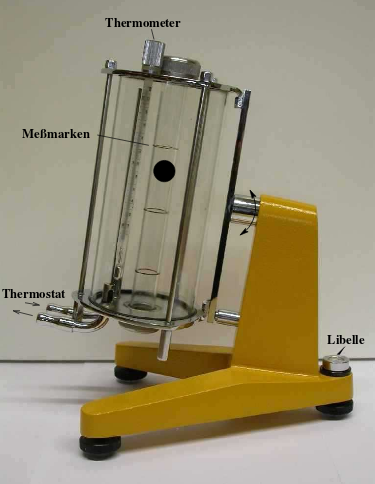
\includegraphics[width=7.50cm, height=9.50cm]{V207_Kugelfall-Viskosimeter_Hoeppler.png}
  \caption{Kugelfall-Viskosimeter\cite{anleitung01}}
  \label{fig:Aufbau}
\end{figure}

\input{"Auswertung.tex"}

\newpage
\printbibliography
\end{document}


\section{Auswertung}
\subsection{Bestimmung der Winkelrichtgröße und des Eigenträgheitmomentes der Drillachse}
Für die Bestimmung der Winkelrichtgröße wurde folgende Formel verwendet:
\begin{equation}
  D = \frac{\lvert F \rvert \cdot \lvert r \rvert}{\varphi}
\end{equation}

Unsere Messergebenisse der Winkel und der jeweilig wirkenden Kraft sind in Tabelle 1 eingetragen.

\begin{table}
  \centering
  \caption{Wirkende Kraft in N in Abhängigkeit des Drehwinkels bei verschiedenen Abständen.}
  \label{tab:data1}
  \begin{tabular}{c c c c c}
    \toprule Abstand in m & $\frac{1}{3} \pi$ & $\frac{2}{3} \pi$ & $ \pi$ & $\frac{4}{3} \pi$ \\
    \midrule
    0.10 & 0.31 & 0.61 & 0.89  & 1.20 \\
    0.15 & 0.20 & 0.40 & 0.595 & 0.89 \\
    0.20 & 0.16 & 0.30 & 0.44  & 0.59 \\
    \bottomrule
  \end{tabular}
\end{table}

Mithilfe der Messdaten werden die jeweiligen Winkelrichtgrößen berechnet und gemittelt,
sodass sich folgender Wert für die "statische" Winkelrichtgröße ergibt:

\begin{equation}
  D_{stat} = (0.0291 \pm 0.0003) \symup{Nm}
\end{equation}

Die Winkelrichtgröße kann auch dynamisch bestimmt werden. Die Messergebnisse dazu befinden sich
in Tabelle 2. Zur Bestimmung von $D_{dyn}$ wird in einem Graphen $T^2$ gegen $a^2$ aufgetragen,
wobei $a$ dem jeweiligen Abstand zum Drillachsenmittelpunkt $\lvert r \rvert$ entspricht und $T$
der jeweilig gemessenen Schwingungsdauer. Mittels linearer Regression wird dann die Steigung $m$ sowie
der y-Achsenabschnitt $b$ berechnet. Mithilfe dieser Werte wird dann ebenfalls die
Winkelrichtgröße mit folgender Formel berechnet:

\begin{equation}
  D_{dyn} = \frac{8\pi^2 \cdot m_{zyl}}{m}
\end{equation}

Der Fehler ergibt sich dabei mithilfe Gauß´scher Fehlerrechnung aus folgender Formel:

\begin{equation}
  \sigma_{D_{dyn}} = \frac{8 \pi^2 \cdot m_{zyl}}{m^2} \cdot \sigma_m
\end{equation}

\begin{table}
  \centering
  \caption{Schwingungsdauern bei jeweiligen Abständen.}
  \label{tab:data2}
  \begin{tabular}{c c c c }
    \toprule $a \, \,  in \,\, m$ & $a^2 \,\, in \,\,  m^2$ & $T \,\, in \,\, s$ & $T^2 \,\, in  \,\, s^2$ \\
    \midrule
    0.0500 & 0.0025 & 2.79867 &  7.8325\\
    0.1000 & 0.0100 & 3.61067 &  13.037\\
    0.1245 & 0.0155 & 4.12933 &  17.051\\
    0.1504 & 0.0226 & 4.71533 &  22.234\\
    0.1751 & 0.0306 & 5.29200 &  28.005\\
    0.2000 & 0.0400 & 5.84000 &  34.106\\
    0.2261 & 0.0511 & 6.49133 &  42.137\\
    0.2505 & 0.0628 & 7.10800 &  50.524\\
    0.2740 & 0.0751 & 7.69600 &  59.228\\
    0.3000 & 0.0900 & 8.33733 &  69.511\\
    \bottomrule
  \end{tabular}
\end{table}

\begin{figure}
  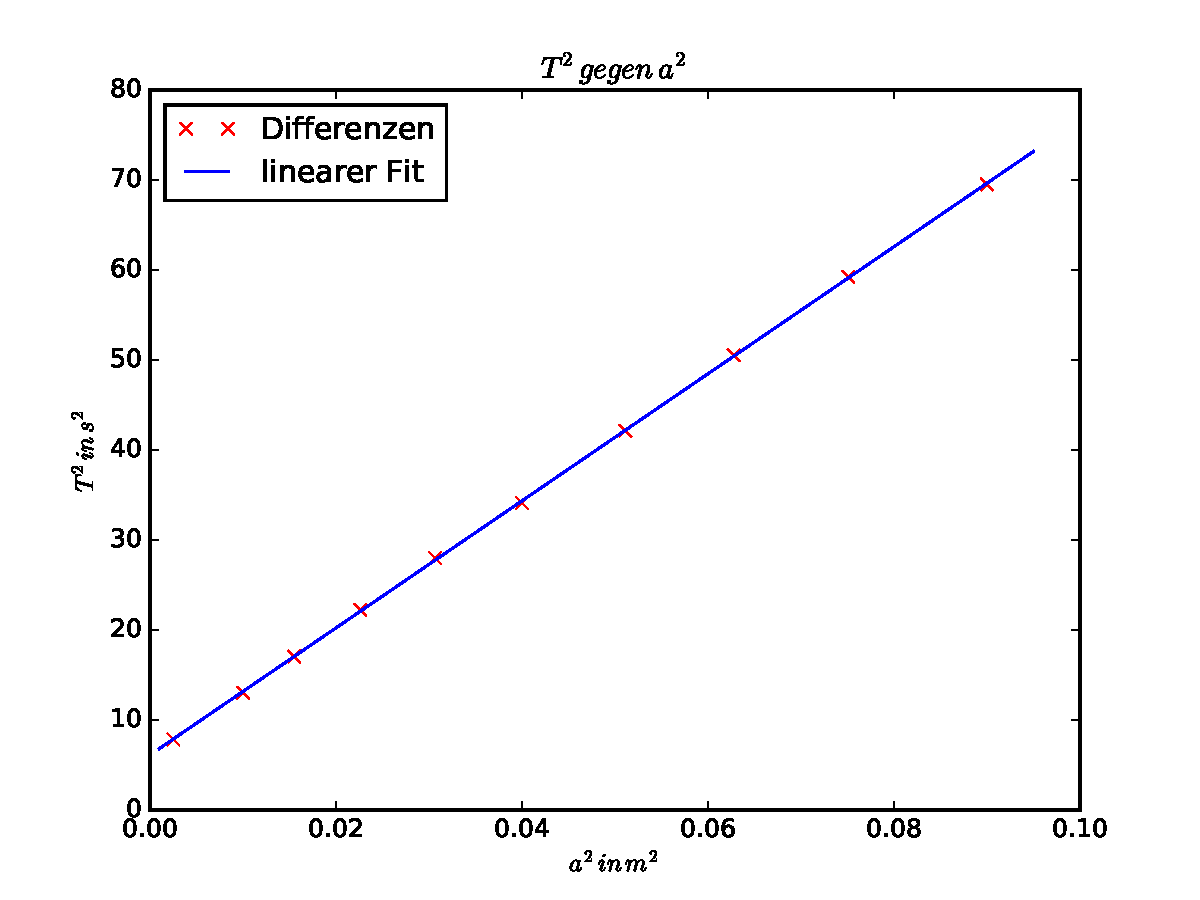
\includegraphics[width=\textwidth]{plot1.pdf}
  \caption{Die Quadrate der Schwingungsdauer gegenüber den Abstandsquadraten}
\end{figure}

Die Regression wird dabei von Python durchgeführt, indem an folgende Funktion gefittet wird.
Die Parameter $C_1$ und $C_2$ entsprechen dabei der Steigung und dem y-Achsenabschnitt:

\begin{align}
  T^2 &= C_1 * a^2 + C_2 \\
  C_1 &= m \\
  C_2 &= b
\end{align}

Die Steigung der Regressionsgerade beträgt $m = (706 \pm 2) \frac{s^2}{m^2}$ und
der y-Achsenabschnitt hat einen Wert von $b = (6.12 \pm 0.09) s^2$. So ergibt sich für
die "dynamische" Winkelrichtgröße folgender Wert:

\begin{equation}
  D_{dyn} = (0.02925 \pm 0.00008) \symup{Nm}
\end{equation}

Zu sehen ist, dass $D_{dyn}$ im Fehlerbereich von $D_{stat}$ liegt, dies aber anders herum nicht
gilt. Da $D_{dyn}$ den geringeren Fehler hat, wird im folgenden mit diesem Wert weitergerechnet.

Mithilfe von $D_{dyn}$ und des y-Achsenabschnittes von Abbildung 1 können nun mit folgenden Formeln
auch das Trägheitsmoment der Drillachse und der Fehler bestimmt werden:

\begin{align}
  I_D        &= I_{ges} - 2 \cdot I_{Z} - I_{Stange}\\
             &= \frac{b \cdot D_{dyn}}{4 \pi^2} - 2 \cdot I_{Z} - I_{Stange}\\
  \sigma_I   &= \sqrt{ \left( \frac{D_{dyn}}{4\pi^2} \cdot \sigma_b \right) ^2 + \left( \frac{b}{4\pi^2} \cdot \sigma_{D_{dyn}} \right) ^2}
\end{align}

Die Trägheitsmomente von Zylinder und Stange müssen vorher noch berechnet werden und hinterher abgezogen werden.
Dabei ergeben sich für $I_{Z}$ und $I_{Stange}$ folgende Werte:

\begin{align}
  I_Z        &= m_{zylinder} \cdot \left( \frac{R_Z^2}{4} + \frac{H_Z^2}{12} \right)\\
  I_{Stange} &= \frac{1}{12} \cdot m_{Stange} \cdot H_{Stange}^2
\end{align}

Bei $R_Z$ und $H_Z$ handelt es sich dabei um Radius und Höhe des Zylinders. Da wir in unserer Formel
den y-Achsenabschnitt verwenden, muss der Steinersche Satz \eqref{eqn:Steiner} nicht beachtet werden, da wir sozusagen
mit einer Schwingungsdauer bei $r=0$ rechnen.
Mit dem obigen y-Achsenabschnitt ergibt sich dann für das Trägheitsmoment der Drillachse folgender Wert:

\begin{equation}
  I_D = (0.0045 \pm 0.0007) \symup{kg m^2}
\end{equation}

\subsection{Bestimmung der Trägheitsmomente zwei verschiedener Körper}
Im folgenden Abschnitt wird das Trägheitsmoment einer homogenen Kugel sowie einer
homogenen Zylinders sowohl theoretisch über Abmessung und Masse sowie experimentell über
die Schwingungsdauer bestimmt und danach verglichen.

\subsubsection{Trägheitsmoment einer homogenen Kugel}
Vor dem Start der Messungen wurden zuerst sowohl Masse als auch Durchmesser der Kugel ermittelt.
Dabei wird beides als fehlerfrei angenommen:

\begin{align}
  r_K &= 0.06883 \symup{m} \\
  m_{Kugel} &= 0.33821 \symup{kg}
\end{align}

Mit diesen Werten lässt sich das "theoretische" Trägheitsmoment wie folgt bestimmen:

\begin{equation}
  I_{Kugel,theo} = \frac{2}{5} m_{Kugel} \cdot r_K^2 = 0.00154 \,\, \symup{kg m^2}
\end{equation}

Als nächstes wird das Trägheitsmoment über die Schwingungsdauer bestimmt. Die gemessenen Werte
sind in Tabelle 3 eingetragen.

\begin{table}
  \centering
  \caption{Schwingungsdauern der homogenen Kugel}
  \begin{tabular}{c c c c c c c c c c c}
    \toprule $Messung$ & $1$ & $2$ & $3$ & $4$ & $5$ & $6$ & $7$ & $8$ & $9$ & $10$ \\
    \midrule $Dauer [s]$ & 7.50 & 7.50 & 7.47 & 7.44 & 7.50 & 7.41 & 7.50 & 7.47 & 7.56 & 7.47\\
    \bottomrule
  \end{tabular}
\end{table}

Für die Schwingungsdauer werden die Werte noch durch 5 geteilt und gemittelt. Wir erhalten somit einen Wert von :

\begin{equation}
  T_{Kugel} = (1.4964 \pm 0.0026) \symup{s}
\end{equation}

Damit ergibt sich für das Trägheitsmoment folgender Wert:

\begin{equation}
  I_{Kugel,exp} = \frac{T^2 D_{dyn}}{4\pi^2} - I_D = (0.00154 \pm 0.00007) \symup{kg m^2}
\end{equation}

Der Fehler errechnet sich wie folgt mithilfe der Gauß´schen Fehlerfortpflanzung:

\begin{equation}
  \sigma_I = \sqrt{(2T \frac{D_{dyn}}{4\pi^2} \cdot \sigma_T)^2 + (\frac{T^2}{4\pi^2} \cdot \sigma_{D_{dyn}})^2}
    \label{eqn:sigma}
\end{equation}

Verwendet wird dabei die dynamisch bestimmte Winkelrichtgröße, da dieser Größe der selbige
Messprozess zugrunde liegt, den wir auch bei der Bestimmung der Trägheitsmomente über die
Schwingungsdauer verwendet haben.

\subsubsection{Trägheitsmoment eines homogenen Zylinders}

Die Messwerte für die Schwingungsdauern finden sich in Tabelle 4. Die Rechnungen sind dabei analog
zu denen der homogenen Kugel.

\begin{align}
  r_Z &= 0.04012  \symup{m} \\
  h_Z &= 0.13990  \symup{m} \\
  m_Z &= 1.00580  \symup{kg}
\end{align}

\begin{equation}
  I_{Zylinder,theo} = \frac{1}{2} m_Z \cdot r_Z^2 = 0.000809 \,\, \symup{kg m^2}
\end{equation}

\begin{table}
  \centering
  \caption{Schwingungsdauern des homogenen Zylinder}
  \begin{tabular}{c c c c c c c c c c c}
    \toprule $Messung$ & $1$ & $2$ & $3$ & $4$ & $5$ & $6$ & $7$ & $8$ & $9$ & $10$ \\
    \midrule $Dauer [s]$ & 5.22 & 5.28 & 5.28 & 5.25 & 5.28 & 5.22 & 5.28 & 5.22 & 5.25 & 5.25\\
    \bottomrule
  \end{tabular}
\end{table}

Für die Schwingungsdauer erhalten wir somit einen Wert von:

\begin{equation}
  T_{Zylinder} = (1.0506 \pm 0.0017) \symup{s}
\end{equation}

Damit errechnet sich für das Trägheitsmoment und dessen Fehler \eqref{eqn:sigma} folgender Wert:

\begin{equation}
  I_{Zylinder,exp} = (0.00070 \pm 0.00007)  \symup{kg m^2}
\end{equation}

\newpage

\subsection{Das Trägheitsmoment einer Holzpuppe in zwei verschiedenen Positionen}

Als letzter Teil der Messungen soll das Trägheitsmoment eine Holzpuppe in zwei verschiedenen
Positionen bestimmt werden. In Position 1 sind die beiden Arme seitlich ausgestreckt und
bei Position 2 sind der rechte Arm sowie das rechte Bein nach vorne ausgestreckt.

%Hier noch Referenz für Sebastian

\subsubsection{Abschätzung des Trägheitsmomentes aus den Abmessungen}
In der folgenden Tabelle sind alle Abmessungen der Puppe eingetragen. Die Indizes entsprechen
dabei dem entsprechendem Körperteil [t = Torso, k = Kopf, a = Arm, b = Bein].

\begin{table}
  \centering
  \caption{Abmessungen der Holzfigur in Metern}
  \begin{tabular}{c c c c c c c c}
    \toprule $r_t$ & $h_t$ & $r_k$ & $h_k$ & $r_a$ & $h_a$ & $r_b$ & $h_b$ \\
    \midrule 0.023034 & 0.13114 & 0.015805 & 0.071 & 0.1002 & 0.17864 & 0.01136 & 0.20042 \\
    \bottomrule
  \end{tabular}
\end{table}

Bei den Rechnungen werden die einzelnen Körperteile als Zylinder angenommen. Da die Körperteile
allerdings teilweise erheblich von diesen Formen abweichen kann folgendes jedoch lediglich als
Abschätzung betrachtet werden. Somit macht auch eine Fehlerrechnung in diesem Fall keinen Sinn
und wird in diesem Abschnitt nicht durchgeführt.

Das Gesamtträgheitsmoment entspricht somit einer Summation der Trägheitsmomente der einzelnen
Körperteile. Um die Massen der einzelnen Körperteile zu ermitteln, wurde das Gesamtvolumen der
Figur berechnet und damit die Dichte bestimmt. Mit dem Volumen der einzelnen Körperteile wurden
dann die einzelnen Massen [Tabelle 6] bestimmt:

\begin{table}
  \centering
  \caption{Volumen und Massen der einzelnen Körperteile}
  \begin{tabular}{c | c c}
    \toprule $Objekt$ & $Volumen [cm^3]$ & $Masse [kg]$ \\
    \midrule
    Torso & 0.0004373 & 0.134536 \\
    Kopf  & 0.0001110 & 0.034293 \\
    Arm   & 0.0001125 & 0.034679 \\
    Bein  & 0.0001625 & 0.050011 \\
  \end{tabular}
\end{table}

\newpage

Für Position 1 gilt somit folgende Formel:

\begin{align}
  I_{ges} &= I_T + I_K + 2 \cdot I_A + 2 \cdot I_B - I_D\\
          &= \frac{1}{2} m_t r_t^2 + \frac{1}{2} m_k r_k^2 + 2 \cdot (m_a(\frac{r_a^2}{4} + \frac{h_a^2}{12}) + m_a(r_t + \frac{h_a}{2})^2) \\
          &+ 2 \cdot (\frac{1}{2} m_b r_b^2 + m_b(\frac{r_b}{2})^2)
\end{align}

Position 2 wird analog berechnet, allerdings wird vorab noch der Abstand der Mittelpunkte von
ausgestrecktem Arm und Bein zur Drehachse bestimmt:

\begin{align}
  \increment_a = \sqrt{(r_t + r_a)^2 + \frac{h_a^2}{4}} \\
  \increment_b = \sqrt{(r_t + r_b)^2 + \frac{h_b^2}{4}}
\end{align}

\begin{align}
  I_{ges} &= I_T + I_K + I_A + I_B - I_D\\
          &= \frac{1}{2} m_t r_t^2 + \frac{1}{2} m_k r_k^2 + (\frac{1}{2} m_a r_a^2 + m_a (r_a + r_t)^2) \\
          &+ (\frac{1}{2} m_b r_b^2 + m_b (\frac{r_t}{2})^2) + (m(\frac{r_b^2}{4} + \frac{h_b^2}{12}) + m_b\increment_2^2) \\
          &+ (m(\frac{r_a^2}{4} + \frac{h_a^2}{12}) + m_a\increment_1^2)
\end{align}

Somit ergeben sich folgende Trägheitsmomente:

\begin{align}
  I_{ges,pos1} = 0.001117 \,\, \symup{kg m^2} \\
  I_{ges,pos2} = 0.001251 \,\, \symup{kg m^2}
\end{align}

\subsubsection{Brechnung der Trägheitsmomente anhand der experimentellen Daten}

Wie zuvor kann nun das Trägheitsmoment auch anhand der experimentell ermittelten Daten (Tabelle 7) bestimmt
werden:

\begin{align}
  T_{pos1} &= (1.1284 \pm 0.0029) \symup{s} \\
  T_{pos2} &= (1.4096 \pm 0.0032) \symup{s}
\end{align}

Der angegebenen Fehler für die Trägheitsmomente errechnet sich nach \eqref{eqn:sigma}.
Somit ergeben sich für die Trägheitsmomente folgende Werte:

\begin{align}
  I_{pos1} &= (0.00083 \pm 0.00007) \symup{kg m^2} \\
  I_{pos2} &= (0.00136 \pm 0.00007) \symup{kg m^2}
\end{align}

\begin{table}
  \centering
  \caption{Schwingungsdauer der beiden Positionen der Holzpuppe}
  \begin{tabular}{c c | c c}
    \toprule $5T_{pos1} [s]$ & $T_{pos1} [s]$ & $5T_{pos2} [s]$ & $T_{pos2} [s]$ \\
    \midrule
    5.63 & 1.126 & 6.07 & 1.394 \\
    5.62 & 1.124 & 7.06 & 1.412 \\
    5.59 & 1.118 & 7.06 & 1.412 \\
    5.63 & 1.126 & 7.04 & 1.408 \\
    5.60 & 1.120 & 7.10 & 1.420 \\
    5.72 & 1.144 & 7.03 & 1.406 \\
    5.62 & 1.124 & 7.13 & 1.426 \\
    5.63 & 1.126 & 7.00 & 1.400 \\
    5.72 & 1.144 & 7.09 & 1.418 \\
    5.66 & 1.132 & 7.00 & 1.400 \\
    \bottomrule
  \end{tabular}
\end{table}

\newpage

\section{Diskussion}

Die Abweichung der dynamischen Winkelrichtgröße zur statischen Winkelrichtgröße beträgt lediglich
ca. $0.6 \%$, somit scheint hier kein systematischer Fehler vorzuliegen. Für die weiteren Berechnungen
wurde in diesem Fall $D_{dyn}$ verwendet, da dieser den kleineren Fehler hatte.

Die Abweichung der experimentell und theoretisch berechneten Werte der beiden Figuren ist mit einer nahezu
nicht vorhandenen Abweichung bei dem homogenen Zylinder ziemlich gering, während sich bei der homogenen Kugel eine
Abweichung von ca. 14 $\%$ ergibt. Allerdings kann davon ausgegangen
werden, dass die theoretischen Werte für beide Objekte näher an den tatsächlichen Werten sind, da
die Abmessungen relativ genau bestimmt werden konnten.

Bei den beiden Figurpositionen erhält man bei Position 1 eine Abweichung von ca. 26 $\%$ und bei Position 2 eine
Abweichung von ca. 9 $\%$. Diese Abweichungen können
überraschend als ziemlich gering angesehen werden, da die Abmessungen der Figuren und die anschließende
Abschätzung aufgrund der stark idealisierten Werte eher als ziemlich ungenau betrachtet werden müssen.
Somit wurde im Vorfeld der Messung ein weitaus größerer Fehler erwartet.

Ein mögliche Fehlerquelle bei den Messungen ist vermutlich das Messen mithilfe einer Stoppuhr,
da hier Faktoren wie zum Beispiel die menschliche Reaktionszeit mit reinspielen.

\newpage

\printbibliography

\end{document}
